\documentclass[12pt,t,aspectratio=169]{beamer}
\usepackage{graphicx}
\setbeameroption{hide notes}
\setbeamertemplate{note page}[plain]
\usepackage{listings}

\input{header.tex}

%%%%%%%%%%%%%%%%%%%%%%%%%%%%%%%%%%%%%%%%%%%%%%%%%%%%%%%%%%%%%%%%%%%%%%
% end of header
%%%%%%%%%%%%%%%%%%%%%%%%%%%%%%%%%%%%%%%%%%%%%%%%%%%%%%%%%%%%%%%%%%%%%%

% title info
\title{QTL mapping \\ in MAGIC populations \\ with R/qtl2}
\subtitle{}
\author{\href{https://kbroman.org}{Karl Broman}}
\institute{Biostatistics \& Medical Informatics, UW{\textendash}Madison}
\date{\href{https://kbroman.org}{\tt \scriptsize \color{foreground} kbroman.org}
\\[-4pt]
\href{https://github.com/kbroman}{\tt \scriptsize \color{foreground} github.com/kbroman}
\\[-4pt]
\href{https://twitter.com/kwbroman}{\tt \scriptsize \color{foreground} @kwbroman}
\\[2pt]
\scriptsize {\lolit Slides:} \href{https://bit.ly/msu2019-12}{\tt \scriptsize
  \color{foreground} bit.ly/msu2019-12}
}


\begin{document}

% title slide
{
\setbeamertemplate{footline}{} % no page number here
\frame{
  \titlepage

  \vfill \hfill \includegraphics[height=6mm]{Figs/cc-zero.png} \vspace*{-3mm}

  \note{These are slides for a talk that I gave at the MAGIC
    workshop in Cambridge, UK, on 23 July 2019; revised and expanded
    for a talk at Michigan State University on 12 Dec 2019.

    Source: {\tt https://github.com/kbroman/Talk\_MSU2019} \\
    Slides: {\tt https://bit.ly/msu2019-12}
}
} }



\begin{frame}[c]{}

\vspace*{-1mm} \hspace*{-2mm}
\figw{Figs/inbredmice.jpg}{1.2}

\end{frame}


\begin{frame}{}

\vspace*{18mm}

\centerline{
\begin{minipage}[t]{50mm}
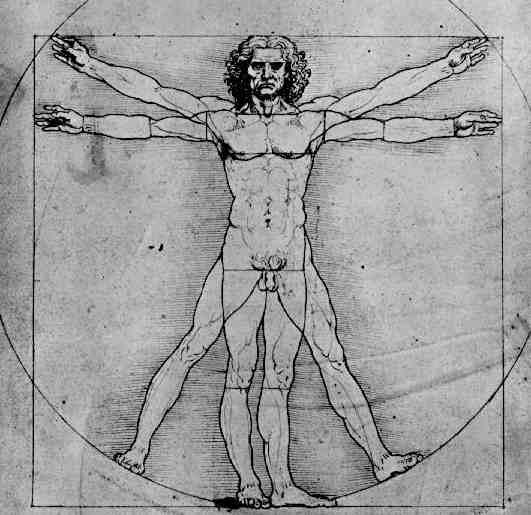
\includegraphics[height=50mm]{Figs/da-vinci-man.jpg}
\end{minipage}
\hspace{15mm}
\begin{minipage}[t]{50mm}
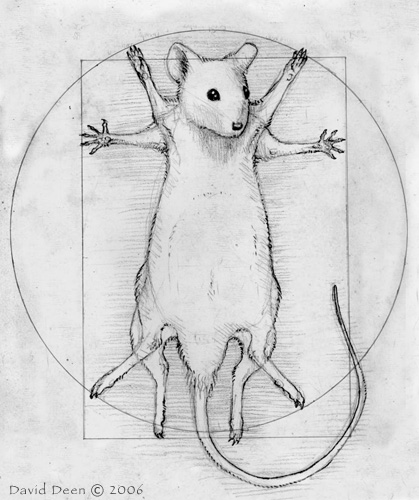
\includegraphics[height=50mm]{Figs/vitruvian_mouse.jpg}
\hspace{5mm}
\href{http://daviddeen.com}{\scriptsize \lolit \tt daviddeen.com}
\end{minipage}
}
\end{frame}


\begin{frame}[c]{Intercross}
\figw{Figs/intercross.pdf}{1.0}
\end{frame}





\begin{frame}[c]{QTL mapping}

\vspace{5mm}
\figh{Figs/lodcurve_insulin_with_effects.pdf}{0.75}
\end{frame}


\begin{frame}[c]{Congenic line/NIL}

\figh{Figs/congenic.pdf}{0.95}

\end{frame}



\begin{frame}[c]{Improving precision}

  \vspace{-20mm}

  \bbi
\item more recombinations
\item more individuals
\item more precise phenotype
\item lower-level phenotypes
\bi
\item transcripts, proteins, metabolites
  \ei
  \ei

\end{frame}



\begin{frame}[c]{Genome-scale phenotypes}

\vspace*{5mm}

\figh{Figs/mouse_on_chips.png}{0.75}
\hfill
\href{https://biochem.wisc.edu/faculty/attie}{\scriptsize \lolit Alan
  Attie} \hspace{8mm}

\end{frame}




\begin{frame}[c]{Advanced intercross lines}

  \figh{Figs/ail.pdf}{0.9}

\end{frame}


\begin{frame}[c]{Recombinant inbred lines}

  \figh{Figs/rilines.pdf}{0.9}

\end{frame}


\begin{frame}[c]{Collaborative Cross}

  \figh{Figs/ri8.pdf}{0.9}

\end{frame}



\begin{frame}[c]{Heterogeneous stock}

  \vspace{2mm}

  \figh{Figs/hs.pdf}{0.9}

\end{frame}


\begin{frame}[c]{MAGIC is magic}

\bbi
\item Genetic diversity

\item High-precision mapping

\item Predictable linkage disequilibrium

\item Phenotype replicates to reduce individual variation

\item Pool phenotypes from multiple labs, environments, treatments

\item Genotype once

\onslide<2->{\item \hilit Cool name}

\ei

\end{frame}






\begin{frame}{MAGIC lines}

 \vspace{5mm}

  \figw{Figs/valdar_genet2006.png}{0.9}

  \vspace{20mm}

\hfill {\footnotesize \href{http://www.genetics.org/content/172/3/1783.full}{\lolit Valdar et al., Genetics 172:1783, 2006}}

\onslide<2->{
  \small {\hilit

  \vspace*{-24mm}
\hspace*{30mm} combine \hspace*{18mm} mix \hspace*{29mm} fix}
}

\onslide<3->{
\vspace*{10pt}
\hspace*{8mm}
How many?
}

\onslide<4->{
\vspace*{8pt}
\hspace*{8mm}
Which?
}

\onslide<5->{
\vspace*{-35pt}
\hspace*{60mm}
How long?
}

\onslide<6->{
\vspace*{-12pt}
\hspace*{100mm}
How?
}

\end{frame}



\begin{frame}[c]{The goal}

Identify QT\only<1>{L}\only<2->{\vhilit G}

\bbi

\item Power
\item Mapping precision
\onslide<3>{\item Estimate QTL allele frequencies}

\ei

\end{frame}




\begin{frame}[c]{Principles}

\bbi

\item Avoid population structure
\item Tradeoff between {\hilit power for \emph{de novo\/} discovery}
  and {\hilit mapping precision}
\item More QTL to find $ \ \Rightarrow \ $ more QTL getting in the way?
\item More QTL alleles $ \ \Rightarrow \ $ less information about each
\item Are QTL alleles common or rare?

\ei

\end{frame}



\begin{frame}{How many founders?}

\vspace{8mm}

  \begin{columns}

    \begin{column}{0.5\textwidth}
      {\hilit More}

{\small
\bi
\item More general use
\item More QTL
\item Greater precision
\item Estimate allele frequencies
\item Haplotype analysis in founders
  \ei
}

    \end{column}

    \begin{column}{0.5\textwidth}
      {\hilit Fewer}

{\small
\bi
\item Lower residual variance
\item Greater power for a particular QTL?
\item Better power for epistasis
\item Rare alleles are less rare
\ei
}
    \end{column}


  \end{columns}


\end{frame}



\begin{frame}[c]{Which founders?}

  \bbi
\item Diverse
\item Interesting
\item No breeding problems
\item Balanced: star phylogeny
  \ei

\end{frame}


\begin{frame}[c]{How much mixing?}

  \bbi
  \item More mixing $ \ \Rightarrow \ $ Greater mapping precision
\item ...but lower power for \emph{de novo\/} mapping
\item Potential for population structure, missing alleles
\item \hilit Random mating or curated mating?
\item \hilit Start with many random cross directions?
  \ei

\end{frame}


\begin{frame}[c]{Selfing or DH?}

\bbi
\item Inbreeding gives added recombination
\item But not so much as at the mixing stage
\item \hilit If doubled haploids are feasible, use them
  \ei

\end{frame}




\begin{frame}[c]{Sharing is also key}

\bbi
\item The greatest power of MAGIC comes from sharing
  \bi
\item[] \hilit Pooling data, exploring multiple environments/treatments
  \ei

\item Common software needs
  \bi
\item[] \hilit Analysis software, database infrastructure
  \ei

\item Many students need to learn the same stuff
  \bi
\item[] \hilit Joint training opportunities
  \ei

  \ei

\end{frame}




\begin{frame}[c]{19 years of R/qtl}

\figw{Figs/rqtl_lines_code.pdf}{0.95}

\end{frame}




\begin{frame}{R/qtl cross types}

\bbi
\item backcross{\lolit , doubled haploids, haploid}

\item intercross

\item 2-way RIL {\lolit by selfing or sibling mating}

\item phase-known 4-way cross
\ei

\end{frame}






\begin{frame}[c]{}

\figh{Figs/rqtl2_3d.png}{0.9}


\end{frame}



\begin{frame}{R/qtl2 cross types}

\vspace*{10mm}

\bi
\item backcross, doubled haploids, haploid

\item intercross

\item 2-, 4-, 8-, 16-way RIL by selfing

\item 2-, 4-, 8-way RIL by sibling mating

\item 2-, 3-, 8-way advanced intercross

\item 6- and 19-way MAGIC

\item Diversity Outbred (DO) mice

\item F$_1$ of DO $\times$ inbred

\item general RIL or AIL
\ei

\end{frame}










\begin{frame}{Data files}

\includegraphics[width=0.8\textwidth]{Figs/phefile.pdf}

\only<2->{
  \vspace*{-50mm}
  \hspace*{15mm}
  \includegraphics[width=0.8\textwidth]{Figs/genfile.pdf}
}


\only<3->{
  \vspace*{-50mm}
  \hspace*{30mm}
  \includegraphics[width=0.8\textwidth]{Figs/fgfile.pdf}
}

\only<4->{
  \vspace*{-60mm}
  \hspace*{45mm}
  \includegraphics[width=0.4\textwidth]{Figs/pmapfile.pdf}
}


\end{frame}



\begin{frame}[c,fragile]{Control file (json or yaml)}
\begin{semiverbatim} \begin{lstlisting}[escapechar=!,]
{
  "description": "Arabidopsis MAGIC data, Gnan et al (2014)",
  !\color{foreground}{"crosstype": "magic19",}!
  "sep": ",",
  "na.strings": ["-", "NA"],
  "comment.char": "#",
  !\color{foreground}{"geno": "arabmagic_geno.csv",}!
  "founder_geno": "arabmagic_foundergeno.csv",
  "gmap": "arabmagic_pmap_tair9.csv",
  "pmap": "arabmagic_pmap_tair9.csv",
  "pheno": "arabmagic_pheno.csv",
  !\color{foreground}{"genotypes": {}!
  !\color{foreground}{  "A": 1}!
  !\color{foreground}{  "H": 2}!
  !\color{foreground}{  "B": 3}!
  !\color{foreground}{\},}!
  !\color{foreground}{"geno_transposed": true,}!
  "founder_geno_transposed": true
}
\end{lstlisting} \end{semiverbatim}
\end{frame}


\begin{frame}[c,fragile]{Control file (json or yaml)}
\addtocounter{framenumber}{-1}
\begin{semiverbatim} \begin{lstlisting}[escapechar=!]
{
  "description": "Arabidopsis MAGIC data, Gnan et al (2014)",
  !\color{vhilit}{"crosstype": "magic19",}!
  "sep": ",",
  "na.strings": ["-", "NA"],
  "comment.char": "#",
  !\color{foreground}{"geno": "arabmagic_geno.csv",}!
  "founder_geno": "arabmagic_foundergeno.csv",
  "gmap": "arabmagic_pmap_tair9.csv",
  "pmap": "arabmagic_pmap_tair9.csv",
  "pheno": "arabmagic_pheno.csv",
  !\color{foreground}{"genotypes": {}!
  !\color{foreground}{  "A": 1}!
  !\color{foreground}{  "H": 2}!
  !\color{foreground}{  "B": 3}!
  !\color{foreground}{\},}!
  !\color{foreground}{"geno_transposed": true,}!
  "founder_geno_transposed": true
}
\end{lstlisting} \end{semiverbatim}
\end{frame}



\begin{frame}[c,fragile]{Control file (json or yaml)}
\addtocounter{framenumber}{-1}
\begin{semiverbatim} \begin{lstlisting}[escapechar=!]
{
  "description": "Arabidopsis MAGIC data, Gnan et al (2014)",
  !\color{foreground}{"crosstype": "magic19",}!
  "sep": ",",
  "na.strings": ["-", "NA"],
  "comment.char": "#",
  !\color{vhilit}{"geno": "arabmagic_geno.csv",}!
  "founder_geno": "arabmagic_foundergeno.csv",
  "gmap": "arabmagic_pmap_tair9.csv",
  "pmap": "arabmagic_pmap_tair9.csv",
  "pheno": "arabmagic_pheno.csv",
  !\color{foreground}{"genotypes": {}!
  !\color{foreground}{  "A": 1}!
  !\color{foreground}{  "H": 2}!
  !\color{foreground}{  "B": 3}!
  !\color{foreground}{\},}!
  !\color{foreground}{"geno_transposed": true,}!
  "founder_geno_transposed": true
}
\end{lstlisting} \end{semiverbatim}
\end{frame}



\begin{frame}[c,fragile]{Control file (json or yaml)}
\addtocounter{framenumber}{-1}
\begin{semiverbatim} \begin{lstlisting}[escapechar=!]
{
  "description": "Arabidopsis MAGIC data, Gnan et al (2014)",
  !\color{foreground}{"crosstype": "magic19",}!
  "sep": ",",
  "na.strings": ["-", "NA"],
  "comment.char": "#",
  !\color{foreground}{"geno": "arabmagic_geno.csv",}!
  "founder_geno": "arabmagic_foundergeno.csv",
  "gmap": "arabmagic_pmap_tair9.csv",
  "pmap": "arabmagic_pmap_tair9.csv",
  "pheno": "arabmagic_pheno.csv",
  !\color{vhilit}{"genotypes": {}!
  !\color{vhilit}{  "A": 1}!
  !\color{vhilit}{  "H": 2}!
  !\color{vhilit}{  "B": 3}!
  !\color{vhilit}{\},}!
  !\color{foreground}{"geno_transposed": true,}!
  "founder_geno_transposed": true
}
\end{lstlisting} \end{semiverbatim}
\end{frame}



\begin{frame}[c,fragile]{Control file (json or yaml)}
\addtocounter{framenumber}{-1}
\begin{semiverbatim} \begin{lstlisting}[escapechar=!]
{
  "description": "Arabidopsis MAGIC data, Gnan et al (2014)",
  !\color{foreground}{"crosstype": "magic19",}!
  "sep": ",",
  "na.strings": ["-", "NA"],
  "comment.char": "#",
  !\color{foreground}{"geno": "arabmagic_geno.csv",}!
  "founder_geno": "arabmagic_foundergeno.csv",
  "gmap": "arabmagic_pmap_tair9.csv",
  "pmap": "arabmagic_pmap_tair9.csv",
  "pheno": "arabmagic_pheno.csv",
  !\color{foreground}{"genotypes": {}!
  !\color{foreground}{  "A": 1}!
  !\color{foreground}{  "H": 2}!
  !\color{foreground}{  "B": 3}!
  !\color{foreground}{\},}!
  !\color{vhilit}{"geno_transposed": true,}!
  "founder_geno_transposed": true
}
\end{lstlisting} \end{semiverbatim}
\end{frame}




\begin{frame}[fragile,c]{Reading data into R}


\begin{center} \begin{minipage}[c]{11.7cm} \begin{semiverbatim}
\lstset{basicstyle=\large}
\begin{lstlisting}[linewidth=11.7cm]
library(qtl2)
arab <- read_cross2("arab_magic.json")
\end{lstlisting}
\end{semiverbatim} \end{minipage} \end{center}


\onslide<2>{
\vfill
\hfill \begin{minipage}[c]{6cm}

  \small
  {\color{title} 19-way Arabidopsis MAGIC} \\
  Kover et al. (2009) PLoS Genet \\
  Gnan et al. (2014) Genetics \\
  {\tt github.com/rqtl/qtl2data}

\end{minipage}
}

\end{frame}


\begin{frame}[c]{Data diagnostics}


\hfill \begin{minipage}{11.7cm}
{\lolit See} Broman et al. (2019) Cleaning genotype data from \\
{\color{background} See} Diversity Outbred mice. G3 9:1571--1579 \\[12pt]
{\color{background} See See} \href{https://doi.org/10.1534/g3.119.400165}{doi: 10.1534/g3.119.400165}
\end{minipage}

\end{frame}



\begin{frame}[c]{Genotype reconstruction}


\only<1>{\figw{Figs/geno_reconstruct.pdf}{0.95}}
\only<2>{\figw{Figs/geno_reconstruct_B.pdf}{0.95}}

\end{frame}




\begin{frame}[c,fragile]{Genotype reconstruction}

\begin{center} \begin{minipage}[c]{11.5cm} \begin{semiverbatim}
\begin{lstlisting}[linewidth=11.5cm]
gmap <- insert_pseudomarkers(arab$gmap, step=0.2, stepwidth="max")
pmap <- interp_map(gmap, arab$gmap, arab$pmap)

pr <- calc_genoprob(arab, gmap, error_prob=0.002, cores=24)
\end{lstlisting}
\end{semiverbatim} \end{minipage} \end{center}

\end{frame}



\begin{frame}[c]{Genome scan}

\only<1>{\figw{Figs/scan_hk.pdf}{1.0}}
\only<2>{\figw{Figs/scan_lmm.pdf}{1.0}}
\only<3>{\figw{Figs/scan_loco.pdf}{1.0}}

\end{frame}

\begin{frame}[c]{Genome scan}

\figw{Figs/scan_seedwt.pdf}{1.0}

\end{frame}


\begin{frame}[c,fragile]{Genome scan}

\begin{center} \begin{minipage}[c]{11.3cm} \begin{semiverbatim}
\begin{lstlisting}[linewidth=11.3cm]
out_hk <- scan1(pr, arab$pheno, cores=24)

operm_hk <- scan1perm(pr, arab$pheno, n_perm=1000, cores=24)

k <- calc_kinship(pr, cores=24)
out_lmm <- scan1(pr, arab$pheno, k, cores=24)

k_loco <- calc_kinship(pr, "loco", cores=24)
out_loco <- scan1(pr, arab$pheno, k_loco, cores=24)
\end{lstlisting}
\end{semiverbatim} \end{minipage} \end{center}

\end{frame}



\begin{frame}[c]{SNP association scan}

\only<1>{\figw{Figs/snp_asso.pdf}{1.0}}
\only<2>{\figw{Figs/snp_asso_B.pdf}{1.0}}
\only<3>{\figw{Figs/snp_asso_B_logp.pdf}{1.0}}

\end{frame}



\begin{frame}[c]{SNP association scan}

\only<1>{\figw{Figs/snp_asso_C.pdf}{1.0}}
\only<2>{\figw{Figs/snp_asso_C_logp.pdf}{1.0}}

\end{frame}


\begin{frame}[c,fragile]{SNP association scan}

\begin{center} \begin{minipage}[c]{11.3cm} \begin{semiverbatim}
\begin{lstlisting}[linewidth=11.3cm]
snp_pr <- genoprob_to_snpprob(pr, arab)

out_snps <- scan1(snp_pr, arab$fruit, cores=24)
\end{lstlisting}
\end{semiverbatim} \end{minipage} \end{center}

\end{frame}





\begin{frame}[c]{QTL effects}

\only<1>{\figw{Figs/coef_fl.pdf}{1.0}}
\only<2>{\figw{Figs/blup_fl.pdf}{1.0}}

\end{frame}



\begin{frame}[c]{QTL effects}

\figw{Figs/blup_sw.pdf}{1.0}

\end{frame}


\begin{frame}[c,fragile]{QTL effects}

\begin{center} \begin{minipage}[c]{11.3cm} \begin{semiverbatim}
\begin{lstlisting}[linewidth=11.3cm]
fl_peak <- max(out_hk, pmap, lodcolumn="fruit_length")
fl_pr <- pull_genoprobpos(pr, pmap, fl_peak$chr, fl_peak$pos)

fl_fit1 <- fit1(fl_pr, arab$pheno[,"fruit_length"])
fl_blup <- fit1(fl_pr, arab$pheno[,"fruit_length"], blup=TRUE)
\end{lstlisting}
\end{semiverbatim} \end{minipage} \end{center}

\end{frame}









\begin{frame}{Goals}

  \bbi
\item Genotype reconstructions from external software

\item General models for RIL and AIL

\item Sequencing-based genotype data

\item Multiple-QTL models

\item QTL $\times$ environment interactions

\item Interactive data visualization
  \ei

\end{frame}




\begin{frame}[c]{}

\Large

Slides: \href{https://bit.ly/msu2019-12}{\tt bit.ly/msu2019-12} \quad
\includegraphics[height=5mm]{Figs/cc-zero.png}

\vspace{7mm}

\href{https://kbroman.org}{\tt \lolit kbroman.org}

\vspace{7mm}

\href{https://kbroman.org/qtl2}{\tt kbroman.org/qtl2}

\vspace{7mm}

\href{https://github.com/kbroman}{\tt \lolit github.com/kbroman}

\vspace{7mm}

\href{https://twitter.com/kwbroman}{\tt \lolit @kwbroman}


\end{frame}

\end{document}
